\documentclass[11pt,a4paper]{article}

% ------------------------------------------------------------
% LinuxPulse project report
% Compile from the repository root with:
%   pdflatex docs/report.tex
% ------------------------------------------------------------

\usepackage[a4paper,margin=25mm]{geometry}
\usepackage[T1]{fontenc}
\usepackage{lmodern}
\usepackage{microtype}
\usepackage{graphicx}
\usepackage{float}
\usepackage{booktabs}
\usepackage{array}
\usepackage{enumitem}
\usepackage{xcolor}
\usepackage{hyperref}
\usepackage{listings}
\usepackage{caption}

\hypersetup{
    colorlinks=true,
    linkcolor=blue!55!black,
    urlcolor=blue!55!black,
    citecolor=blue!55!black,
    pdftitle={LinuxPulse Project Report},
    pdfauthor={LinuxPulse Team}
}

\setlength{\parskip}{0.45em}
\setlength{\parindent}{0pt}
\setlist[itemize]{leftmargin=1.5em,itemsep=0.2em}
\setlist[enumerate]{leftmargin=1.7em,itemsep=0.2em}

\definecolor{codegray}{RGB}{245,246,248}
\lstset{
    basicstyle=\ttfamily\small,
    backgroundcolor=\color{codegray},
    frame=single,
    breaklines=true,
    columns=fullflexible
}

\title{\textbf{LinuxPulse}\\
\large Real-Time System Monitoring Dashboard}
\author{Team: Mentally Unstable\\[0.4em]
\textit{Project Report}}
\date{November 2026}

\begin{document}
\maketitle

\begin{abstract}
LinuxPulse is a desktop system-monitoring application that collects operating-system
telemetry and presents it through a graphical dashboard. It provides live views of
CPU, memory, swap, system load, processes, historical measurements, and resource
alerts. This report describes the project at a system level, documents the
visualization work and its verification, and reserves a section for an additional
team member's contribution.
\end{abstract}

\tableofcontents
\newpage

\section{Introduction}

Operating systems expose a range of measurements that help users understand
resource utilization and identify processes that may be consuming excessive
resources. LinuxPulse brings selected measurements together in a single desktop
interface and updates the displayed information periodically.

The application was run and verified on a MacBook running macOS (Darwin,
arm64). The project also includes platform-aware collection support for Linux
and macOS.

\subsection{Objectives}

The main objectives of LinuxPulse are:
\begin{itemize}
    \item Collect CPU, memory, swap, load-average, and process information.
    \item Normalize collected measurements into a consistent representation.
    \item Maintain historical samples and calculate summary statistics.
    \item Display current measurements and their history through interactive
          dashboard views.
    \item Identify threshold violations and present alerts to the user.
    \item Handle unavailable or incomplete measurements without treating
          missing values as valid zero measurements.
\end{itemize}

\section{System Overview and Architecture}

LinuxPulse is organized into components with distinct responsibilities.

\begin{description}[style=nextline]
    \item[Collector]
    Obtains system measurements and process information from the host operating
    system using platform-specific collection paths.

    \item[Parser]
    Interprets command output and system data, converting it into structured
    values for downstream processing.

    \item[Analytics]
    Maintains bounded measurement history, calculates averages and peaks,
    identifies top resource-consuming processes, and evaluates alert thresholds.

    \item[Models]
    Provides structured representations used to pass system and analytics data
    through the application.

    \item[Visualization]
    Creates and updates Matplotlib figures used to display time-series and
    resource-utilization information.

    \item[GUI]
    Presents overview, process, analytics, and project-information views.

    \item[Launcher]
    The \texttt{run.sh} script prepares the Python virtual environment,
    installs the declared dependencies, and starts the application.
\end{description}

The overall data flow is:

\begin{center}
\texttt{Operating System}
$\rightarrow$ \texttt{Collector}
$\rightarrow$ \texttt{Parser}
$\rightarrow$ \texttt{Analytics / Models}
$\rightarrow$ \texttt{Visualization}
$\rightarrow$ \texttt{GUI}
\end{center}

\section{Technology Stack}

\begin{table}[H]
\centering
\begin{tabular}{ll}
\toprule
\textbf{Technology} & \textbf{Purpose} \\
\midrule
Python & Application and monitoring logic \\
Tkinter & Desktop graphical user interface \\
Matplotlib & Charts and data visualization \\
Standard Python libraries & Data handling, process coordination, and testing \\
Unix command-line utilities & Platform-specific system data collection \\
\bottomrule
\end{tabular}
\caption{Principal technologies used by LinuxPulse.}
\end{table}

\section{Visualization Implementation}

The visualization layer turns the collected and processed measurements into
readable graphical representations. It is designed to update existing plot
objects as new samples arrive, rather than rebuilding the complete dashboard
for every measurement.

\subsection{Overview visualizations}

The overview presents current CPU, RAM, and swap utilization, system load,
monitoring status, and a metrics index. It also includes historical CPU and
memory charts and a per-core utilization area.

The CPU and memory history charts display changes over time. The memory chart
distinguishes used memory, buffer/cache, and free memory. The dashboard updates
periodically as new samples are received.

\subsection{Analytics visualizations}

The analytics view presents average and peak resource measurements, utilization
history, system load history, top resource consumers, and active alerts. This
view makes it possible to examine trends over the monitoring interval rather
than relying only on the latest sample.

\subsection{Handling unavailable measurements}

A measurement may be unavailable on a particular operating system or data
source. LinuxPulse indicates unavailable per-core CPU data in the interface
instead of displaying fabricated values. During verification on macOS, the
dashboard reported that per-CPU data was not provided by the macOS \texttt{top}
data source. The other dashboard measurements and charts continued to operate.

\section{Application Verification}

The integrated application was launched on macOS using the repository's
\texttt{run.sh} script. The script created a virtual environment and installed
the dependencies declared in \texttt{requirements.txt}. The dashboard then
opened and displayed live system information.

\subsection{Functional checks}

The following behavior was visually checked during the application run:
\begin{itemize}
    \item Overview: CPU, RAM, swap, system load, monitoring status, and
          historical charts were displayed.
    \item Processes: the process table, CPU-based process ranking, task counts,
          and recent alerts were displayed.
    \item Analytics: average and peak measurements, utilization histories,
          top resource consumers, and active alerts were displayed.
    \item Project information: the introduction page displayed project and
          host information.
\end{itemize}

\subsection{Automated tests}

The complete discovered unit-test suite was executed with:

\begin{lstlisting}
python3 -m unittest discover -s tests -v
\end{lstlisting}

The run completed successfully with 55 tests passing and no failures.

\begin{table}[H]
\centering
\begin{tabular}{lr}
\toprule
\textbf{Test area} & \textbf{Tests passed} \\
\midrule
Analytics & 21 \\
Collector & 10 \\
Parser & 20 \\
Visualization & 4 \\
\midrule
\textbf{Total} & \textbf{55} \\
\bottomrule
\end{tabular}
\caption{Automated test results from the integrated project.}
\end{table}

\textit{Note:} The test counts above reflect the successful test run recorded
during project verification.

\section{Screenshots}

The repository contains screenshots of the integrated application. The
following figures are included when the report is compiled from the repository
root and the image files are present under \texttt{assets/screenshots/}.

\begin{figure}[H]
    \centering
    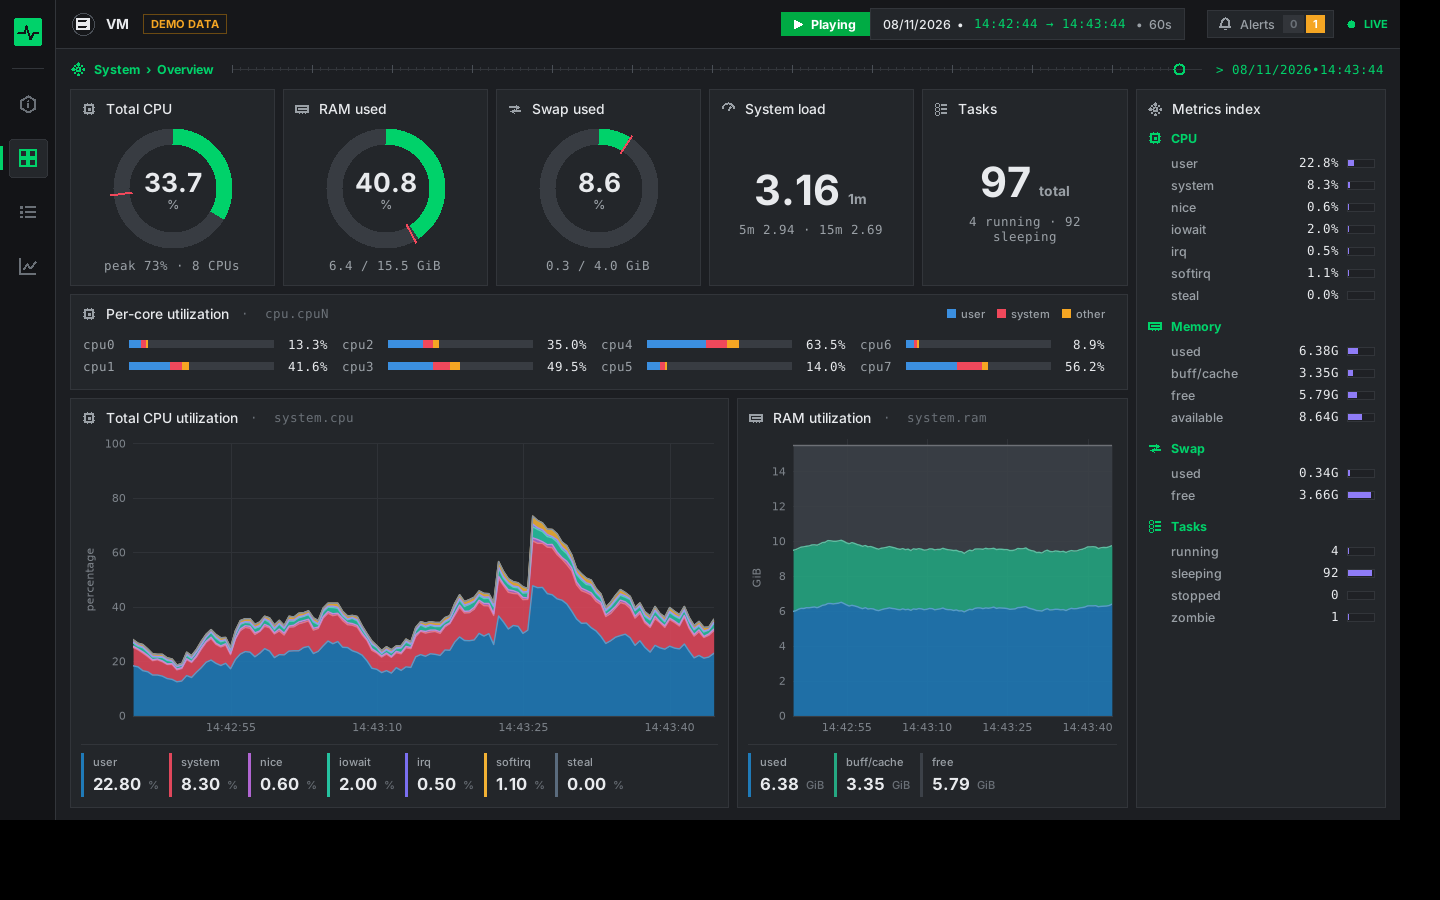
\includegraphics[width=\textwidth]{assets/screenshots/overview.png}
    \caption{LinuxPulse overview dashboard.}
    \label{fig:overview}
\end{figure}

\begin{figure}[H]
    \centering
    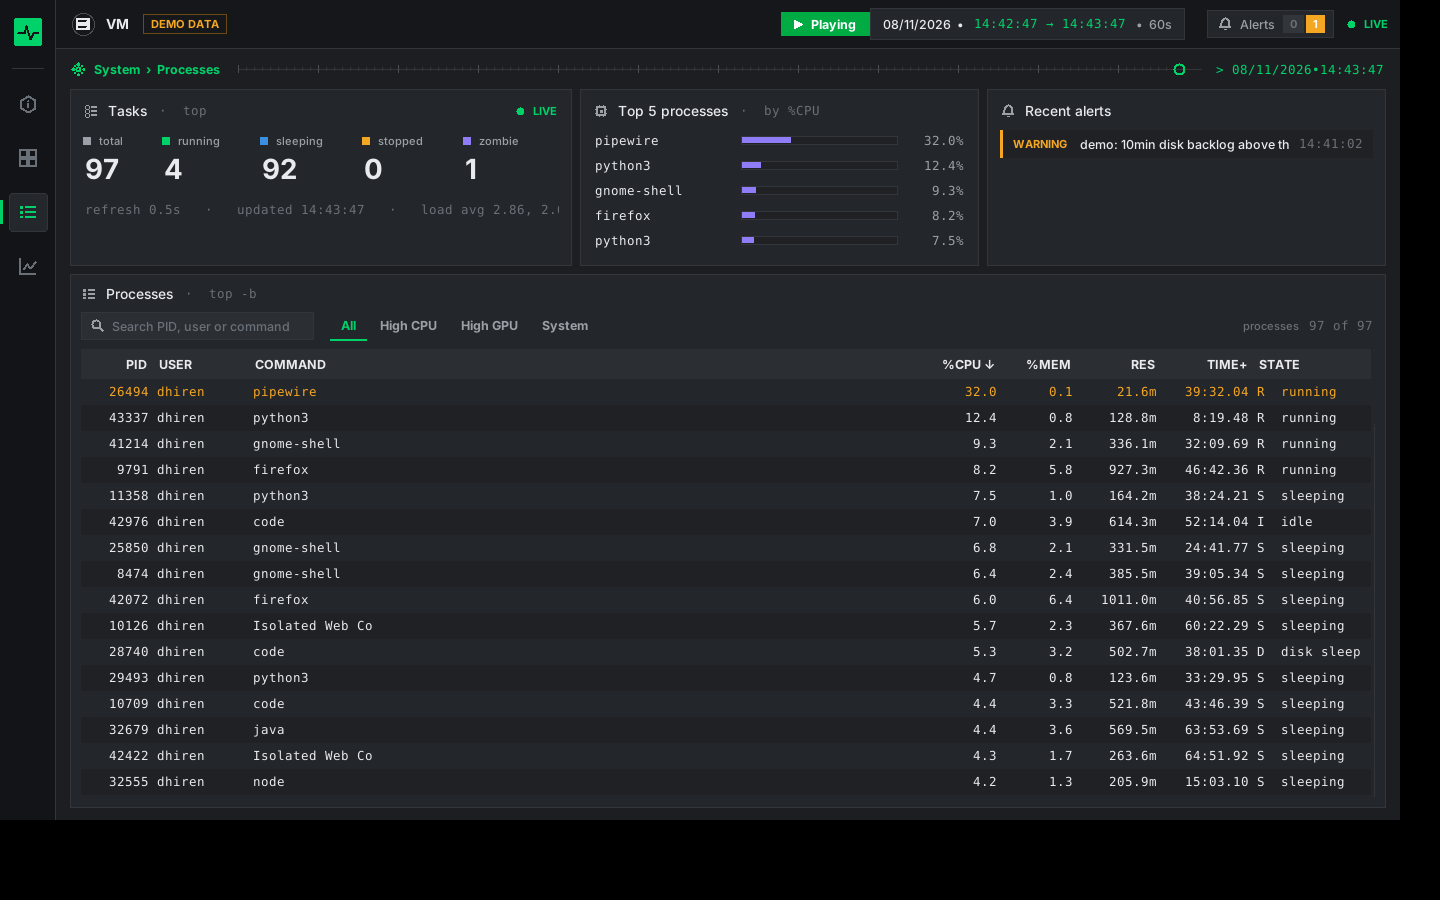
\includegraphics[width=\textwidth]{assets/screenshots/processes.png}
    \caption{Process monitoring view.}
    \label{fig:processes}
\end{figure}

\begin{figure}[H]
    \centering
    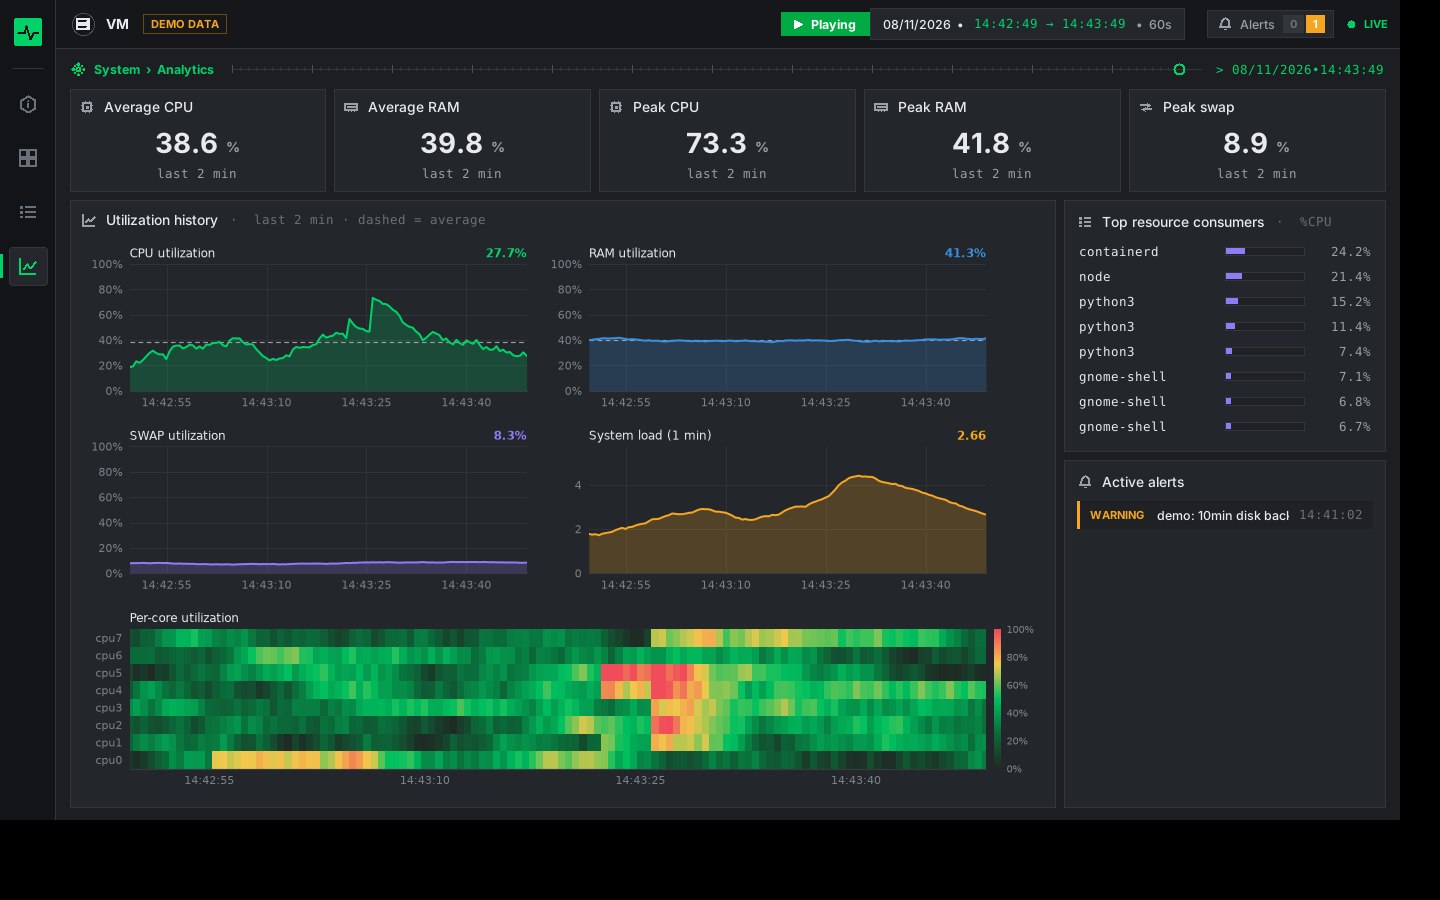
\includegraphics[width=\textwidth]{assets/screenshots/analytics.png}
    \caption{Analytics and historical utilization view.}
    \label{fig:analytics}
\end{figure}

\section{Limitations and Future Improvements}

The availability and detail of system measurements depend on the operating
system and the underlying collection utility. In the macOS verification run,
per-core CPU measurements were unavailable from the selected data source.
Potential future improvements include:
\begin{itemize}
    \item Adding or evaluating a platform-specific source for per-core CPU data
          on macOS.
    \item Expanding integration and cross-platform testing.
    \item Evaluating dashboard responsiveness and memory use during longer
          monitoring sessions.
    \item Improving the presentation of unavailable measurements and collection
          errors where appropriate.
\end{itemize}

\section{Team Contributions}

\subsection{Visualization and verification}

\textbf{Contributor: Pavan Nandan Gudipudi}

Work covered the visualization component and its verification, including:
\begin{itemize}
    \item Implementing Matplotlib-based system monitoring plots.
    \item Supporting CPU, RAM, and swap history visualization.
    \item Updating plot data as new measurements arrive.
    \item Handling empty input, missing values, unequal input lengths, and
          bounded recent history in visualization tests.
    \item Documenting the visualization design, testing strategy, and
          performance observations.
    \item Verifying the integrated dashboard on macOS and running the complete
          automated test suite.
\end{itemize}

\subsection{Additional team member contribution --- placeholder}

% ============================================================
% PLACEHOLDER FOR THE OTHER TEAM MEMBER:
% Replace the prompts below with their name, responsibility,
% implementation details, and testing/results. Keep this
% section until their contribution has been added.
% ============================================================

\textbf{Contributor:} \textit{[Add name]}

\textbf{Area of responsibility:} \textit{[Add module or responsibility]}

\textbf{Work completed:}
\begin{itemize}
    \item \textit{[Describe the implementation or assigned work.]}
    \item \textit{[Describe relevant design decisions or features.]}
    \item \textit{[Describe tests, validation, or results.]}
\end{itemize}

\textbf{Evidence / references:} \textit{[Add relevant files, figures, commits,
or test results.]}

\section{Conclusion}

LinuxPulse brings system collection, parsing, analytics, visualization, and a
desktop interface together in one application. During the recorded macOS
verification, the overview, processes, analytics, and project-information
views operated, and the automated test suite completed with 55 passing tests.
The project provides a foundation for real-time system monitoring while
retaining explicit handling for measurements that are unavailable from a
particular platform data source.

\end{document}
